%\thispagestyle{myheadings}
\section{Invited Talk: Julia Hirschberg}
\index{Hirschberg, Julia}


\begin{center}
\begin{Large}
{\bfseries\Large Truth or Lie? Spoken Indicators of Deception in Speech}\vspace{1em}\par
\end{Large}

%% \begin{center}
%%   \begin{tabular}{m{1in}b{1in}}
%%     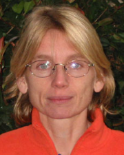
\includegraphics[width=1in]{content/monday/cortes-headshot.png}
%%     & {\bfseries Corinna Cortes} \newline Google Research, NY
%%   \end{tabular}
%% \end{center}

\daydateyear, 9:00--10:00 \vspace{1em}\\
\PlenaryLoc \\
\vspace{1em}\par
%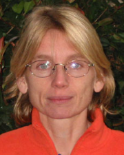
\includegraphics[height=100px]{content/monday/cortes-headshot.png}
\end{center}

\noindent
{\bfseries Abstract:} Detecting deception from various forms of human behavior is a longstanding research goal which is of considerable interest to the military, law enforcement, corporate security, social services and mental health workers. However, both humans and polygraphs are very poor at this task. We describe more accurate methods we have developed to detect deception automatically from spoken language. Our classifiers are trained on the largest cleanly recorded corpus of within-subject deceptive and non-deceptive speech that has been collected. To distinguish truth from lie we make use of acoustic-prosodic, lexical, demographic, and personality features. We further examine differences in deceptive behavior based upon gender, personality, and native language (Mandarin Chinese vs. English), comparing our systems to human performance. We extend our studies to identify cues in trusted speech vs. mistrusted speech and how these features differ by speaker and by listener. Why does a listener believe a lie? 

\vspace{3em}\par 

\vfill
\noindent

{\bfseries Biography:} Julia Hirschberg is Percy K. and Vida L. W. Hudson Professor and Chair of Computer Science at Columbia University. She previously worked at Bell Laboratories and AT\&T Labs where she created the HCI Research Department. She has been editor of Computational Linguistics and Speech Communication, is a fellow of AAAI, ISCA, ACL, ACM, and IEEE, and a member of the National Academy of Engineering. She received the IEEE James L. Flanagan Speech and Audio Processing Award and the ISCA Medal for Scientific Achievement. She currently serves on the IEEE Speech and Language Processing Technical Committee, is co-chair of the CRA-W Board, and has worked for diversity for many years at AT\&T and Columbia. She works on spoken language processing and NLP, studying text-to-speech synthesis, spoken dialogue systems, entrainment in conversation, detection of deceptive and emotional speech, hedging behavior, and linguistic code-switching (language mixing).
\newpage
